%!TEX root = main.tex

% \textbf{Workflow1: $Head Cast \rightarrow Merge Cast \rightarrow Tail Cast$}
% \vspace{-2mm}

We first look at how Alloy compares with
machine algorithms, other crowd algorithms, and inter-expert agreements.  In
the Head Cast, crowdworkers highlight keyword and cluster similar clips via
searching, and in the Tail Cast another set of crowdworkers organizes all remaining clips.

We compare this Workflow 1 to three baselines that are commonly used in the
clustering literature: latent Dirichlet Allocation (LDA) \cite{blei2003latent},
latent semantic analysis (LSA) \cite{deerwester1990indexing}, and TF-IDF
\cite{manning2008introduction,Jones72astatistical}. We also compare against a
hybrid baseline that uses human-identified keyword vectors from the Head Cast.  This aims to test the value of the approach beyond the human identification of keywords by trying to cluster using only the keywords.
In addition to comparing against automatic methods, we also
compare Alloy to a popular crowd based method.
% \joseph{duplicated}
% The baseline systems required different
% parameters as additional inputs (i.e., stopping threshold, number of topics,
% number of dimensions, priors, ..., etc.).  Some of these parameters can be
% time-consuming to fine-tune \cite{chuang2012termite}.  Therefore, for each
% question, we iterated on different parameter combinations for each of the
% baseline systems, and reported the best score to compare with our method.
The evaluation conditions are summarized below:

\begin{itemize}
    \setlength\itemsep{0.0em}

	\item \emph{Workflow1}. The workflow with ten crowdworkers each for
		the Head Cast and the Tail Cast for Q1-Q4. An additional five workers for the Merge Cast for Q5-Q6. Each HIT costs 1 USD.
	\item \emph{TF-IDF}. Weighted cosine similarity as the
		similarity function for the Gather.
		No human-computation was employed.
	\item \emph{Crowd keywords}. Cosine similarity based on worker-highlighted keywords from the Head Cast as the
		similarity function for the Gather.
	\item \emph{LSA}. The LSA model is used as the similarity function for
		the Gather.  No human-computation was employed.
	\item \emph{LDA}. The LDA topic model is used as the similarity function
		for the Gather.  No human-computation was employed.
	\item \emph{Cascade}. A version of Cascade with only one recursion 
    	using the default parameters as described in the paper.
        
\end{itemize}


\subsubsection*{Results}

Alloy introduces a novel approach for providing context in the microtask setting with the sampling mechanism in the Head Cast. We captured  crowdworkers' behavior during the tasks and found that  
nearly all (97.5\%) workers
used the sampling mechanism to gain context beyond the initial four items. On average, each worker sampled 15.1 items
, and more specifically, 11.3\% sampled more than 25 items, 23.8\%
sampled 15\texttildelow 24 items and 62.5\% sampled 5\texttildelow 14 items.

\subsubsection*{Comparing with Machine Algorithms}

On average, the proposed method performed significantly better and more consistent
than all machine baselines (Table~\ref{tab:results}). In the worst case, Alloy
clusters measured 0.058 NMI lower than the inter-annotator agreement, while
the baseline systems measured more than 0.1 NMI lower in most cases.  In a few
cases some baselines also performed well (e.g., LSA performed slightly better on Q5),
but none of them
produced good results consistently across all datasets.  Compared to the
gold-standard clusters, Alloy produced clusters about as close to the
gold-standard clusters as the two human annotators were to each other, despite
the judges' advantages of having a global view of the datasets and multiple
rounds of reading, labeling, and discussion. 
In addition, worker-identified keywords consistently outperformed TF-IDF,
showing that the crowdworkers are extracting keywords in the Head Cast that are
salient for identifying clusters each dataset.
On the two larger datasets (Q5 and Q6), Alloy achieved similar
performance as the four smaller datasets; better
and more consistent comparing to the baseline systems, and near experts
agreement comparing to the gold-standard.

Note that for every machine algorithm baseline we explored multiple parameters
for each of the four questions, (hyper-parameters, number of topics,
stopping threshold), and report the highest scores.  The results of the
baseline algorithms are likely over-fitting to the data, but we wanted to
compare Alloy to these algorithms under their best possible settings \cite{chuang2012termite}.

% The portion of corpus clustered
% after Phase A are 57\%, 82\%, 74\%, 87\% for each question, respectively.  The
% number of remaining clips is small enough to feed into the none distributed
% variant of Phase B without running Merge Cast first.

\subsubsection*{Comparing with Previous Crowd Methods}


\begin{figure}
	\centering
	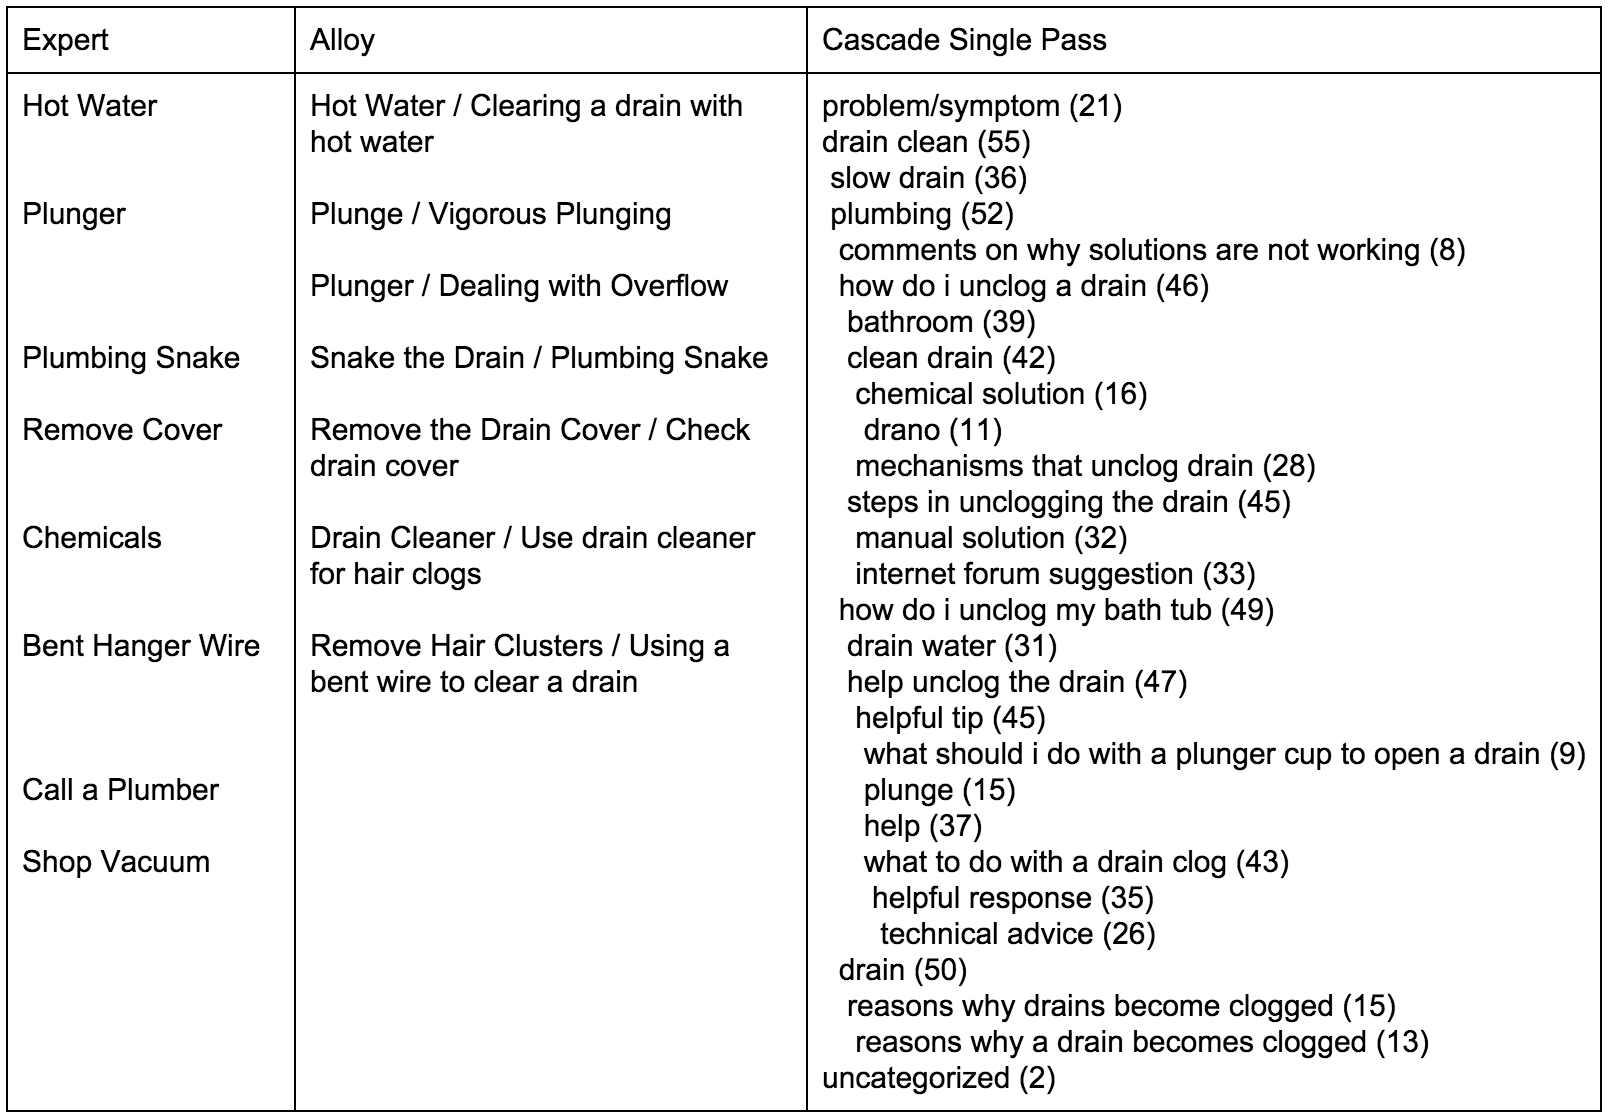
\includegraphics[width=0.9\columnwidth]{Chapters/Alloy/images/bathtub_cats.png}
	\caption{Categories comparison for Q1}
	\label{fig:bathtub_cats}
\end{figure}

%\begin{figure}
%	\centering
%	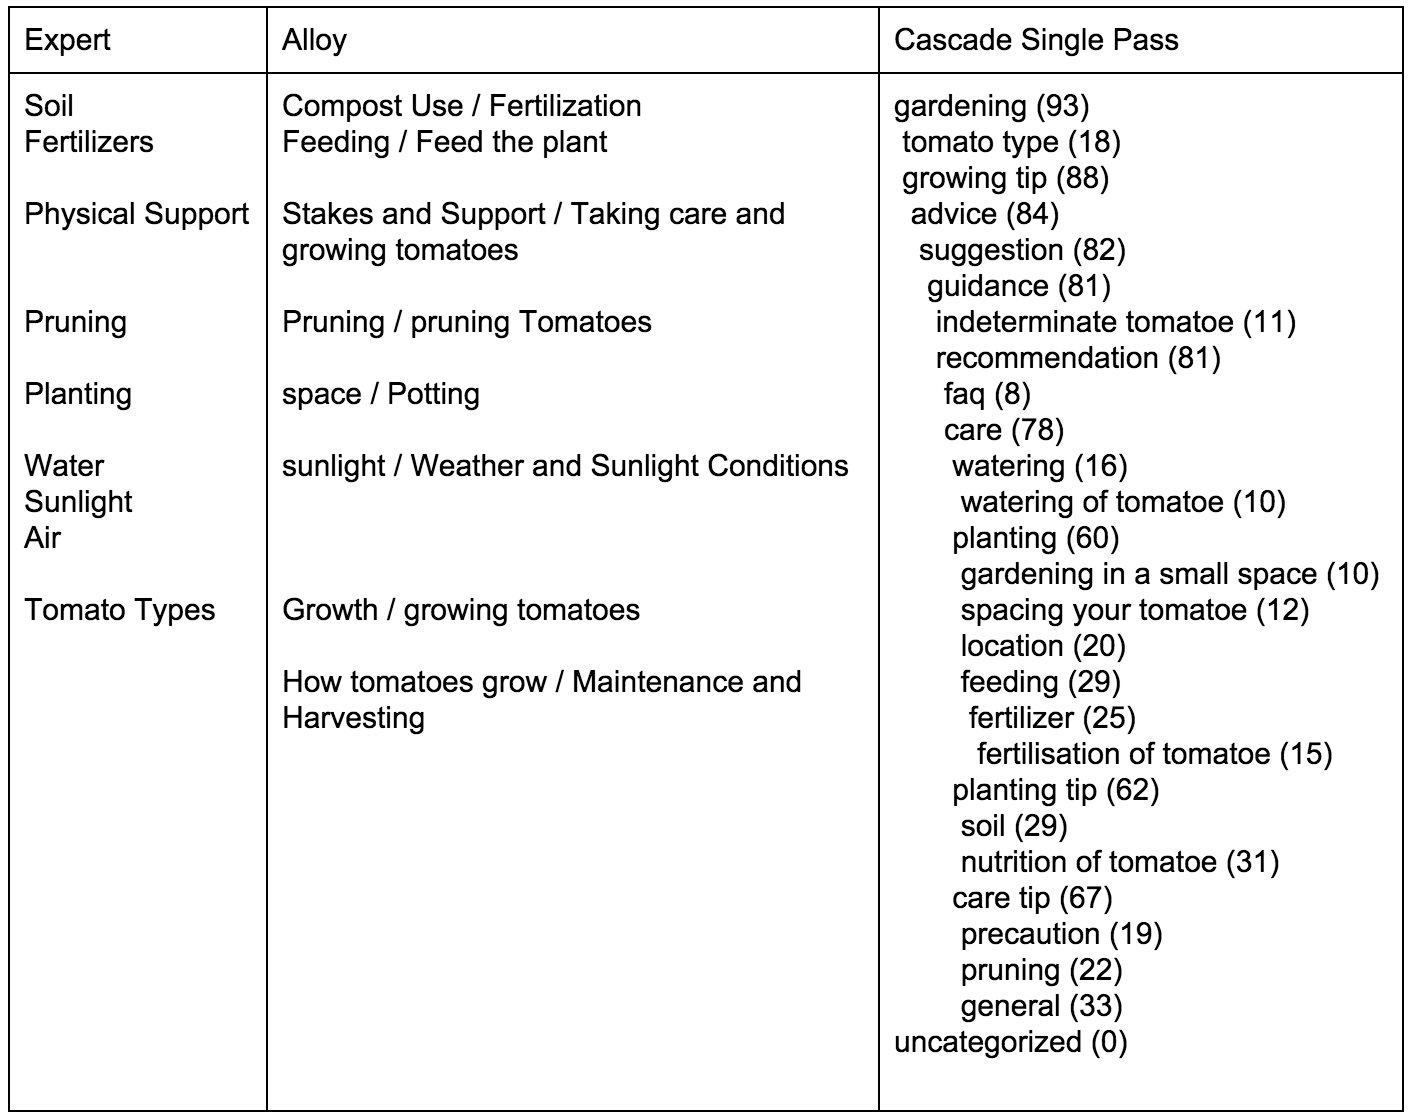
\includegraphics[width=0.9\columnwidth]{images/tomato_cats.png}
%	\caption{Categories comparison for Q2}
%	\label{fig:tomato_cats}
% \end{figure}

We compare Alloy with Cascade using datasets Q1-Q4, a popular crowd-based method for
discovering taxonomies in unstructured data based on overlapping crowd
clusters \cite{chilton2013cascade}.
We implemented a simplified version of Cascade using the parameters
described in the paper, but with only one recursion.  We acknowledge that fine
tuning and multiple recursion might improve Cascade's performance, but the
numbers from our evaluation are consistent with the results reported in the
Cascade paper based on the same metric and similar datasets.

On average, 84\% of categories generated with Alloy were shared with clusters
in the gold standard, versus 50\% for Cascade.  Cascade produced soft
clusters where child clusters did not necessarily have all the items included in
their parents, which breaks the assumptions of using NMI. To produce
a direct comparison, we use the gold standard to greedily extract best
matching, overlapping clusters that cover all items, and evaluated them using
the average F1. In essence, this simulates an omniscient ``oracle'' that gives
Cascade the best possible set of cluster matches, and so is perhaps overly
generous but we wanted to err on the conservative side. The average F1 scores
for each questions using Alloy are .72, .54, .48, .52, and using Cascade are
.50, .48, .42, .39, showing a consistent advantage across questions.
Furthermore, Alloy achieved this better performance at a
lower cost (average \$20 for Alloy vs \$71 for Cascade),
suggesting that machine learning can provide valuable scaling properties.
We show categories created by experts and elicited from the two systems
in Figure~\ref{fig:bathtub_cats} to give a better sense of the datasets and the output.
% and  Figure~\ref{fig:tomato_cats}. 

% \begin{table*}
%   \centering
% 
% \begin{tabular}{ |l|l|p{3in}| }
% \hline
% Expert & Alloy & Cascade Single \\
% \hline
% Hot Water & Hot Water / Clearing a drain with hot water & \\
% Plunger   & Plunge / Vigorous Plunging & \\
%           & Plunger / Dealing with Overflow & \\
% Plumbing Snake & Snake the Drain / Plumbing Snake & \\
% Remove Cover   & Remove the Drain Cover / Check drain cover & \\
% hemicals       & Drain Cleaner / Use drain cleaner for hair clogs & \\
% Bent Hanger Wire & Remove Hair Clusters / Using a bent wire to clear a drain & \\
% Call a Plumber & & \\
% Shop Vacuum & & 
% \multirow{-9}*{
% \begin{minipage}{3in}
% problem/symptom (21)\newline
% drain clean (55)\newline
% \hspace{1mm} slow drain (36)\newline
% \hspace{1mm} plumbing (52)\newline
% \hspace{1mm} \hspace{1mm}  comments on why solutions are not working (8)\newline
%   how do i unclog a drain (46)\newline
%    bathroom (39)\newline
%    clean drain (42)\newline
%     chemical solution (16)\newline
%      drano (11)\newline
%     mechanisms that unclog drain (28)\newline
%    steps in unclogging the drain (45)\newline
%     manual solution (32)\newline
%     internet forum suggestion (33)\newline
%   how do i unclog my bath tub (49)\newline
%    drain water (31)\newline
%    help unclog the drain (47)\newline
%     helpful tip (45)\newline
%      what should i do with a plunger cup to open a drain (9)\newline
%      plunge (15)\newline
%      help (37)\newline
%      what to do with a drain clog (43)\newline
%       helpful response (35)\newline
%        technical advice (26)\newline
%   drain (50)\newline
%    reasons why drains become clogged (15)\newline
%     reasons why a drain becomes clogged (13)\newline
% uncategorized (2)\newline
% \end{minipage}
% } \\[3.1in]
% \hline
% 
% \end{tabular}
%   \caption{Bathtub Categories}
%   \label{tab:bathtub_cats}
% \end{table*}




% \subsection{Crowdworkers}

% The crowdworkers employed to test the proposed method are recruited from Amazon
% Mechanical Turk. With a total of 65 unique workers participated in the
% experiments, 56 of them have IP addresses origin in the United States, 6 of
% them from India, and 3 from other regions. From self-reporting, 40 workers are
% males and 25 workers are females, 8 workers are between the age of 18 to 24, 40
% workers are between the age of 25 to 34, 15 workers are between the age of 35
% to 44, and the rest in other ranges or chose not to report. Each worker is paid
% 1.00 USD for completing one of the two HITs. Therefore, the costs for both
% Workflow2 and Workflow1 is 20.00 USD.

% \begin{table*}
%   \centering
% % question, number of sources, number of clips, number of turkers
%   \begin{tabular}{ c l l l l l }
%     \hline
% 	\tabhead{} &
% 	\tabhead{Phase A Mean} &
% 	\tabhead{Phase A Std. Dev} &
% 	\tabhead{Phase B Mean} &
% 	\tabhead{Phase B Std. Dev} &
% 	\tabhead{ANOVA P-Value} \\
%     \hline

% 	Interface & 4.2270 & 0.6477 & 3.710 & 0.783 & $\sim$ 0.000 \\ 
% 	Instructions & 4.0286 & 0.9592 & 3.786 & 1.001 & $\sim$ 0.156 \\
% 	Difficulty & 3.5099 & 1.0255 & 3.119 & 1.109 & $\sim$ 0.033 \\

%     \hline

%   \end{tabular}
%   \caption{Survey feedback from the crowdworkers.}
%   \label{tab:feedback}
% \end{table*}


% \subsection{Survey feedback from Crowdworkers}
% Upon completion of each HIT, we asked each unique worker to rate the task
% description, interface design, and overall difficulty of the HITs by filling
% out a survey form. We used a 5-point Likert scale, ranging from ``Strongly
% Agree'' (5) to ``Strongly Disagree'' (1) in order to gauge their opinions
% regarding the different features of the HIT. As shown in Table \ref{tab:feedback}, workers
% thought that the interface from Phase A was easier to utilize than interface
% for Phase B (p-value $\sim$ 0.000), with their average response being that they
% agreed that Phase A's interface was easy to use, while Phase B's interface
% was acceptable. There was not a significant difference between their responses
% regarding the instructions, agreeing that for both phases the instructions were
% easy to understand and follow. Finally, workers thought that Phase A was easier
% than Phase B (p-value $\sim$ 0.033), with neither task being considered to be
% particularly easy to complete. 

% We also allowed the Crowdworkers to comment on the HITs, and many of them find
% the clustering process interesting and enjoyable, leaving comments such as
% ``This was an interesting hit. I enjoyed it.'', ``very interesting to name each
% clusters'', and ``This was an interesting study and I actually learned a new
% tip to try and clear a clogged drain.'' 


%\begin{table*}
%  \centering
%% question, number of sources, number of clips, number of turkers
%  \begin{tabular}{ l r r r r r }
%    \hline
%	\tabhead{Questions} &
%	\tabhead{strongly agree} &
%	\tabhead{agree} &
%	\tabhead{neither...} &
%	\tabhead{disagree} &
%	\tabhead{strongly disagree} \\
%    \hline
%    \multicolumn{6}{c}{\tabhead{Phase A}} \\
%    \hline
%	% 54
%	\emph{I find this task easy to complete} & 11\% & 46\% & 31\% & 11\% & 0\% \\
%  
%	% 53
%	\emph{The instructions clearly explain the task} & 34\% & 55\% & 8\% & 4\% & 0\% \\
% 
%	% 54
%	\emph{The user interface is easy to learn and use} & 40\% & 56\% & 4\% & 0\% & 0\% \\
%    \hline
%    \multicolumn{6}{c}{\tabhead{Phase B}} \\
%    \hline
%	% 54
%	\emph{I find this task easy to complete} & 9\% & 45\% & 9\% & 36\% & 0\% \\
%
%	% 53
%	\emph{The instructions clearly explain the task} & 18\% & 55\% & 11\% & 11\% & 11\% \\
%
%	% 54
%	\emph{The user interface is easy to learn and use} & 27\% & 55\% & 11\% & 11\% & 0\% \\
%    \hline
%
%  \end{tabular}
%  \caption{Survey feedback from the crowdworkers.}
%  \label{tab:feedback}
%\end{table*}

